\graphicspath{{../results/figures/regression_analysis/}}
\maketitle


\section{Method}


We build voxelwise brain encoding models that predict BOLD fMRI responses from
the text of naturalistic audio stories.  Eight embedding configurations across
five families are evaluated---from a non-semantic bag-of-words baseline to a
LoRA fine-tuned BERT model reading from middle transformer layers---all fitted
via ridge regression with efficient SVD-based per-voxel regularization selection.



Words are produced at an irregular rate (${\sim}2$--4\,words/s), whereas fMRI
samples uniformly at 0.5\,Hz.  The following three operations, applied
identically across all representation methods, bring both signals onto a common
time grid and account for the sluggish hemodynamic response.


\subsection{Preprocessing}
Let $\bm{E} \in \mathbb{R}^{N \times d}$ denote the word-rate embedding matrix
for a story with $N$ words and embedding dimension $d$.  We resample $\bm{E}$ to
the TR grid using Lanczos sinc interpolation, leveraging the per-word onset
timestamps stored in the dataset, yielding
$\bm{E}_{\mathrm{TR}} \in \mathbb{R}^{256 \times d}$.  Lanczos interpolation
preserves spectral content to a greater degree than nearest-neighbor or linear
resampling, which matters because the BOLD signal occupies a narrow low-frequency
band.



We discard the first 5 TRs (10\,s) to remove scanner equilibration artifacts and
the final 10 TRs (20\,s) to avoid the residual BOLD tail extending past the audio
stimulus, yielding $T = 241$ timepoints per story.  The fMRI response matrices
$\bm{Y}$ are pre-trimmed identically during dataset preparation; no further
trimming is applied to $\bm{Y}$.



The BOLD signal lags neural activity by approximately 4--6\,s.  Rather than
convolving with a fixed hemodynamic response function (HRF), we model the HRF
implicitly by stacking four time-shifted copies of
$\bm{E}_{\mathrm{TR}}[6{:}-10, :]$ (post-trim) at delays
$\delta \in \{1, 2, 3, 4\}$\,TRs:
%
\begin{equation}
  \bm{X} = \bigl[\bm{E}^{(\delta=1)},\; \bm{E}^{(\delta=2)},\;
                  \bm{E}^{(\delta=3)},\; \bm{E}^{(\delta=4)}\bigr]
  \;\in\; \mathbb{R}^{T \times 4d}.
\end{equation}
%
This quadruples the feature dimension and allows the ridge model to learn a
per-voxel hemodynamic filter from data.  Stacking training stories gives
$\bm{X}_{\mathrm{train}} \in \mathbb{R}^{27678 \times 4d}$ and
$\bm{X}_{\mathrm{test}} \in \mathbb{R}^{7108 \times 4d}$.


\subsection{Text Representations}


We compare six text representation methods spanning a broad range of semantic
and contextual richness.
\subsubsection{Baseline Embeddings}
We used three major textual embeddings for baseline analysis, including 

(1)Bag of Words: A \texttt{CountVectorizer} is fit on the union of all training and test stories
to build a vocabulary of ${\approx}12{,}000$ types.  Each word is encoded as a
one-hot sparse vector; after delay stacking the feature dimension is
$4 \times 12{,}000 \approx 48{,}000$.  Because the BoW matrix is
${\sim}99.99\%$ sparse, a dedicated sparse solver is used (Section
\ref{sec:sparse_solver}).



(2) Word2Vec: We use the Google News skip-gram model pretrained on ${\sim}10^{11}$ tokens,
which provides 300-dimensional dense vectors per word.  Out-of-vocabulary words
are mapped to zero vectors.  Final dimensionality: $4 \times 300 = 1{,}200$.



(3) Glove: We use the Stanford 840B Common Crawl GloVe vectors (300-d); lookup is
case-insensitive.  Out-of-vocabulary words are zeroed.  Final dimensionality:
$4 \times 300 = 1{,}200$.

\subsubsection{Contextual Representations with BERT}

We extract contextual word embeddings from \texttt{bert-base-uncased} (12
transformer layers, hidden size $d_h = 768$, 110M parameters).  WordPiece
subword tokens are pooled to one vector per original word by averaging over
subword token positions.  All four BERT-based methods share this tokenization
and pooling step; they differ in (a) how much surrounding context each word
receives, (b) which transformer layers are read out, and (c) whether the
model weights have been fine-tuned on podcast text.


(1) Baseline (reference) BERT: As a reference, each story is split into non-overlapping 128-word chunks that
are fed independently to BERT.  The final layer's hidden state
($\ell = 12$) is used directly.  Words at chunk boundaries receive no context
from adjacent chunks.  Final dimensionality: $4 \times 768 = 3{,}072$.



(2) Enhanced BERT: We apply two modifications over the vanilla baseline to improve the quality of
the contextual signal passed to the ridge model.

\textbf{Sliding-window context.}
Stories are processed with overlapping windows of 256 words and a stride of 128
words (50\% overlap), safely within BERT's 512-token limit
(${\sim}1.3$ tokens/word on average).  Each word appears in up to two windows;
its embeddings are averaged across windows, giving boundary words access to
richer bilateral context and eliminating the context-truncation artifacts of
independent chunking.

\textbf{Multi-layer averaging.}
We average the hidden states of the last four transformer layers
($\ell \in \{9,10,11,12\}$) rather than using only the final layer.  This
\texttt{last4\_mean} strategy blends high-level semantic content captured in the
upper layers with structural and syntactic information retained in lower layers,
and is widely reported to improve downstream representation quality.

Final dimensionality: $4 \times 768 = 3{,}072$.

\subsubsection{Domain Adaptation via LoRA Fine-Tuning}
\label{sec:lora}



(1) LoRA Training Setup (shared across all LoRA variants): To adapt BERT to the podcast domain, we fine-tune \texttt{bert-base-uncased} on
the 81 training stories using Low-Rank Adaptation (LoRA; Hu et al., 2022) with
a masked language modeling (MLM) objective.  LoRA injects trainable rank-$r$
weight updates
$\Delta W = \bm{B}\bm{A} \in \mathbb{R}^{m \times n}$
($r = 32$, scaling $\alpha = 64$, dropout 0.1) into the query, key, value, and
feed-forward projection matrices of every transformer block, while all original
pretrained weights remain \emph{frozen}.  The total number of trainable
parameters is $2rn \ll mn$ per layer, making fine-tuning tractable on the small
podcast corpus (${\approx}157{,}000$ words).

\textbf{Masking schedule.}
We follow the original BERT recipe: 15\% of non-special tokens are selected,
of which 80\% are replaced by \texttt{[MASK]}, 10\% by a random vocabulary
token, and 10\% left unchanged.

\textbf{Training details.}
Stories are segmented into non-overlapping 128-word chunks and tokenized with
\texttt{is\_split\_into\_words=True}.  A random 10\% of chunks is held out for
validation.  We train for 8 epochs with AdamW ($\text{lr} = 2 \times 10^{-5}$,
cosine annealing) on an NVIDIA A100 GPU, saving a checkpoint each epoch and
keeping the one with lowest validation MLM loss.  The best checkpoint occurs at
epoch~5 (val loss 2.157); subsequent epochs show mild overfitting.

The three LoRA variants below all use this same fine-tuned checkpoint.  They
differ \emph{only} in which layers are read out during embedding extraction and,
for LoRA (improved), in the training recipe.



(2) LoRA BERT (last4): Embeddings are extracted from the fine-tuned checkpoint using the same
sliding-window (256 words, stride 128) and \texttt{last4\_mean} pooling
($\ell \in \{9,10,11,12\}$) as Enhanced BERT.  This isolates the effect of
podcast-domain fine-tuning from changes in context or layer selection.



(3) LoRA BERT (improved): This variant modifies the \emph{training} recipe while keeping last4\_mean
extraction.  Two changes are made relative to LoRA (last4):
(i)~\textbf{whole-word masking}: all subword tokens belonging to the same
word are masked together, preventing the model from reconstructing whole words
from visible subword pieces; and
(ii)~\textbf{256-word training chunks}: the chunk size during fine-tuning is
enlarged to 256 words to match the inference window, so the model's
context-length distribution is consistent between training and extraction.



(4) LoRA BERT (mid4): This variant keeps the improved fine-tuned checkpoint but changes the
\textbf{extraction layers} from the last four ($\ell \in \{9,10,11,12\}$) to
the \textbf{middle four} ($\ell \in \{5,6,7,8\}$).  This single change produces
the largest gain across all experiments.

\textit{Why middle layers are superior for brain encoding.}
BERT's 12 transformer layers form a representational hierarchy in which
different levels of linguistic abstraction peak at different depths.  Lower
layers ($\ell \leq 4$) primarily encode surface features: tokenization
boundaries, POS tags, and local morphological patterns.  \textbf{Middle layers
($\ell \approx 5$--$8$)} capture compositional syntactic and semantic structure:
phrase constituency, dependency relations, and thematic role assignments
(Tenney et al., 2019; Jawahar et al., 2019).  Upper layers ($\ell \geq 9$)
are progressively reshaped by the MLM pretraining objective toward predicting
masked tokens, encoding cloze-style lexical predictability rather than abstract
linguistic structure.

The human language network---spanning the left inferior frontal gyrus (LIFG),
superior temporal gyrus (STG), and adjacent association cortex---is organized
around exactly the compositional, multi-word representations that peak in BERT's
middle layers.  The upper layers, by contrast, encode token-prediction signals
that are more localized and task-specific.  Extracting from layers 5--8 therefore
provides a richer match to the spatial profile of cortical language processing,
while the upper layers introduce noise from the MLM objective that weakens the
brain-prediction signal.

Importantly, fine-tuning is still beneficial: extracting mid4\_mean from the
original pretrained BERT (without LoRA adaptation) gives lower correlations than
from the podcast-fine-tuned checkpoint (not shown), indicating that domain
adaptation shifts the middle-layer representations toward the podcast register
even though the gain is not visible in last4 extraction.

\subsection{Ridge Regression}
\label{sec:ridge}

\subsubsection{Modeling}
For each representation and each subject we fit an independent ridge regression
from $\bm{X} \in \mathbb{R}^{T \times p}$ to the voxelwise BOLD responses
$\bm{Y} \in \mathbb{R}^{T \times V}$.  Each column of $\bm{Y}$ is z-scored
per training story to remove run-level baseline shifts; each column of $\bm{X}$
is z-scored globally across all training timepoints.  The ridge estimator is:
%
\begin{equation}
  \hat{\bm{W}}(\lambda) \;=\;
  \underset{\bm{W}}{\arg\min}\;
  \|\bm{Y} - \bm{X}\bm{W}\|_F^2 + \lambda\|\bm{W}\|_F^2
  \;=\;
  \bigl(\bm{X}^\top\bm{X} + \lambda\bm{I}\bigr)^{-1}\bm{X}^\top\bm{Y}.
\end{equation}
%
Test-set performance for each voxel $v$ is evaluated as the Pearson correlation
$r_v$ between the predicted response
$\hat{\bm{y}}_v = \bm{X}_{\mathrm{test}}\hat{\bm{w}}_v$
and the observed BOLD signal $\bm{y}_v$.


For all dense representations we exploit the SVD identity to amortize the cost
of evaluating multiple regularization values.  Given the thin SVD
$\bm{X}_{\mathrm{train}} = \bm{U}\bm{S}\bm{V}^\top$, the ridge solution becomes:
%
\begin{equation}
  \hat{\bm{W}}(\lambda) \;=\;
  \bm{V}\operatorname{diag}\!\left(\frac{s_i}{s_i^2 + \lambda}\right)\bm{U}^\top\bm{Y}.
\end{equation}
%
The SVD is computed once; evaluating a new $\lambda$ requires only an $O(r)$
diagonal rescaling rather than a fresh matrix inversion.  We search over 10
log-spaced values $\lambda \in [10^0, 10^3]$.

\subsubsection{Implementation}

We split the training data temporally into a fit set (80\%) and a validation set
(20\%).  Two SVDs are precomputed outside the voxel loop: one on the fit set for
per-voxel $\lambda$ selection, and one on the full training set for final weight
estimation.  For each voxel independently, we select the $\lambda$ that maximizes
validation-set Pearson correlation, then refit on all training data with that
$\lambda$.  Sharing both SVDs across all voxels means per-voxel $\lambda$
selection incurs no additional SVD cost.



The BoW feature matrix is high-dimensional ($p \approx 48{,}000$) and
${\sim}99.99\%$ sparse, making dense SVD infeasible in memory.  We instead
solve $(\bm{X}^\top\bm{X} + \lambda\bm{I})\bm{W} = \bm{X}^\top\bm{Y}$
using a sparse LU decomposition.  A single global $\lambda$ is chosen by
evaluating a random sample of 200 voxels on a 10\%-held-out fraction of the
training data, avoiding the memory cost of per-voxel selection with a
high-dimensional sparse system.



Voxels are processed in chunks of 500, with BOLD responses streamed from
memory-mapped \texttt{.npy} files to avoid materializing the full
$T \times V$ response matrix simultaneously.  Each training story is
independently z-scored within each chunk to remove scan-session baseline
differences.  Computation is distributed across SLURM array jobs, each
processing a disjoint subset of voxel chunks in parallel; partial results are
merged after all tasks complete.

\section{Main Results}

\begin{table}[htbp]
  \centering
  \caption{Summary of all evaluated representations. Features = $4d$ after
           hemodynamic delay stacking. Solver: \textbf{D} = dense SVD,
           \textbf{S} = sparse LU.}
  \label{tab:methods}
  \begin{tabular}{llcrcc}
    \toprule
    Method & Pretraining & $d$ & Features & Solver & $\lambda$ selection \\
    \midrule
    BoW           & ---                    & ${\sim}12{,}000$ & ${\sim}48{,}000$ & S & Global (200 voxels) \\
    Word2Vec      & Google News (100B)     & 300              & 1{,}200          & D & Per-voxel \\
    GloVe         & Common Crawl (840B)    & 300              & 1{,}200          & D & Per-voxel \\
    Vanilla BERT  & Wikipedia + BooksCorpus & 768             & 3{,}072          & D & Per-voxel \\
    Enhanced BERT & Wikipedia + BooksCorpus & 768             & 3{,}072          & D & Per-voxel \\
    LoRA BERT     & + podcast MLM (8 ep.)  & 768              & 3{,}072          & D & Per-voxel \\
    \bottomrule
  \end{tabular}
\end{table}


\subsection{Ridge Regression Results}
\label{sec:ridge_results}

Table~\ref{tab:results} reports test-set Pearson correlation ($r$) for all
representations on both subjects.  Five summary statistics are shown: mean and
median across all cortical voxels (a global measure of encoding quality),
the 95th and 99th percentile values (capturing the upper tail of
language-responsive voxels), and the single best-voxel correlation.

\begin{table}[htbp]
  \centering
  \caption{Test-set Pearson correlation $r$ per voxel for all methods and
           subjects.  Mean and median are computed over all cortical voxels;
           Top~5\% and Top~1\% denote the 95th and 99th percentiles;
           Best is the single highest-correlation voxel.}
  \label{tab:results}
  \begin{tabular}{llccccc}
    \toprule
    Method & Subj. & Mean $r$ & Median $r$ & Top 5\% $r$ & Top 1\% $r$ & Best $r$ \\
    \midrule
    \multirow{2}{*}{BoW}
      & s2 & 0.0069 & 0.0058 & 0.0343 & 0.0530 & 0.1082 \\
      & s3 & 0.0137 & 0.0107 & 0.0528 & 0.0813 & 0.1526 \\
    \addlinespace
    \multirow{2}{*}{Word2Vec}
      & s2 & 0.0124 & 0.0099 & 0.0485 & 0.0722 & 0.1182 \\
      & s3 & 0.0231 & 0.0180 & 0.0747 & 0.1083 & 0.1720 \\
    \addlinespace
    \multirow{2}{*}{GloVe}
      & s2 & 0.0128 & 0.0099 & 0.0505 & 0.0759 & 0.1327 \\
      & s3 & 0.0219 & 0.0168 & 0.0739 & 0.1080 & 0.1779 \\
    \addlinespace
    \multirow{2}{*}{Vanilla BERT}
      & s2 & 0.0218 & 0.0163 & 0.0743 & 0.1104 & 0.1949 \\
      & s3 & 0.0353 & 0.0269 & 0.1078 & 0.1551 & 0.2870 \\
    \addlinespace
    \multirow{2}{*}{Enhanced BERT}
      & s2 & 0.0349 & 0.0295 & 0.0919 & 0.1341 & 0.2324 \\
      & s3 & 0.0493 & 0.0404 & 0.1255 & 0.1776 & 0.3126 \\
    \addlinespace
    \multirow{2}{*}{LoRA BERT (last4)}
      & s2 & 0.0343 & 0.0288 & 0.0915 & 0.1346 & 0.2356 \\
      & s3 & 0.0489 & 0.0399 & 0.1262 & 0.1791 & 0.3130 \\
    \addlinespace
    \multirow{2}{*}{LoRA BERT (improved)}
      & s2 & 0.0345 & 0.0287 & 0.0933 & 0.1372 & 0.2366 \\
      & s3 & 0.0491 & 0.0398 & 0.1274 & 0.1806 & 0.3163 \\
    \addlinespace
    \multirow{2}{*}{\textbf{LoRA BERT (mid4)}}
      & s2 & \textbf{0.0374} & \textbf{0.0330} & 0.0913 & 0.1330 & 0.2288 \\
      & s3 & \textbf{0.0512} & \textbf{0.0432} & 0.1247 & 0.1802 & 0.3090 \\
    \bottomrule
  \end{tabular}
\end{table}

Several trends emerge.  Within the non-contextual tier, BoW is the weakest
method (mean $r = 0.0069$/$0.0137$ on s2/s3), consistent with its purely
count-based representation lacking any semantic information.  Word2Vec and GloVe
are nearly on par: Word2Vec slightly underperforms GloVe on s2 ($-3\%$) but
slightly outperforms on s3 ($+$5.5\%), reflecting their similar 300-dimensional
distributional semantics despite different training corpora.

Contextual representations show large, consistent gains.  Vanilla BERT raises
mean $r$ on s2 by ${\sim}71\%$ relative to GloVe (0.0218 vs.\ 0.0128) and by
${\sim}61\%$ on s3 (0.0353 vs.\ 0.0219).  Enhanced BERT---with sliding-window
context and multi-layer averaging---adds a further ${\sim}60\%$ gain over Vanilla
BERT on s2 (0.0349 vs.\ 0.0218) and ${\sim}40\%$ on s3 (0.0493 vs.\ 0.0353),
demonstrating the cumulative value of richer context and layer pooling.

LoRA fine-tuning on the podcast corpus with last4 extraction yields essentially
no improvement over Enhanced BERT: s2 performance is slightly lower
(0.0343 vs.\ 0.0349, $-$1.7\%) and s3 is nearly identical
(0.0489 vs.\ 0.0493, $-$0.8\%).  This near-zero delta indicates that adapting
the upper layers to podcast text does not shift the representational geometry
exploited by the ridge model.  An improved training recipe (whole-word masking
and 256-word chunks) showed similarly negligible gains ($+$0.6\% on s2,
$+$0.4\% on s3) with Spearman rank correlation $\rho = 0.977$/$0.984$ between
the two last4 variants, confirming the bottleneck is layer choice, not the
fine-tuning recipe.

By contrast, switching the extraction window to the middle four layers
(\textit{mid4\_mean}, $\ell \in \{5,6,7,8\}$) produces the largest single gain
in the hierarchy: $+$9.1\% on s2 (0.0374 vs.\ 0.0343) and $+$4.7\% on s3
(0.0512 vs.\ 0.0489), corresponding to a $+$193\%/$+$133\% improvement over
GloVe.  The Spearman rank correlation between mid4 and last4 per-voxel CC
vectors drops to $\rho = 0.866$/$0.909$---substantially below the near-perfect
$\rho = 0.977$/$0.984$ between the two last4 variants---confirming that changing
extraction depth genuinely redistributes predictive power to a different set of
brain regions.

Subject~s3 consistently achieves higher correlations than s2 across all methods,
suggesting stronger or more widespread language-responsive BOLD signals.


\subsection{CC Distributions Across Methods}


Figure~\ref{fig:cc_dist} shows the full per-voxel CC distribution for each
method and subject as violin plots.  The distribution is right-skewed for all
methods: the vast majority of voxels have near-zero $r$, while a small
language-responsive tail extends to $r > 0.1$.  Three properties are visible
in the figure.

\textbf{Progressive rightward shift.}
The median and mean shift monotonically across all eight methods, from BoW
through Word2Vec and GloVe to Vanilla BERT and the LoRA variants.  The body of
the violin---representing the bulk of cortical voxels---moves only modestly, but
the upper tail (marked by the dashed Top-5\% threshold) stretches substantially:
from $r_{95} = 0.034$ (BoW, s2) to $r_{95} = 0.091$ (LoRA mid4, s2), a
$+168\%$ gain across the full method hierarchy.

\textbf{Between-method variance compression.}
The spread of the violin narrows for the three LoRA variants, indicating that
fine-tuned models produce more consistent predictions across voxels rather than
outsized gains only in a few.

\textbf{Subject differences.}
Subject~s3's distributions are shifted higher than s2's at every method,
consistent with a larger or more reproducible language-responsive network.

\begin{figure}[htbp]
  \centering
  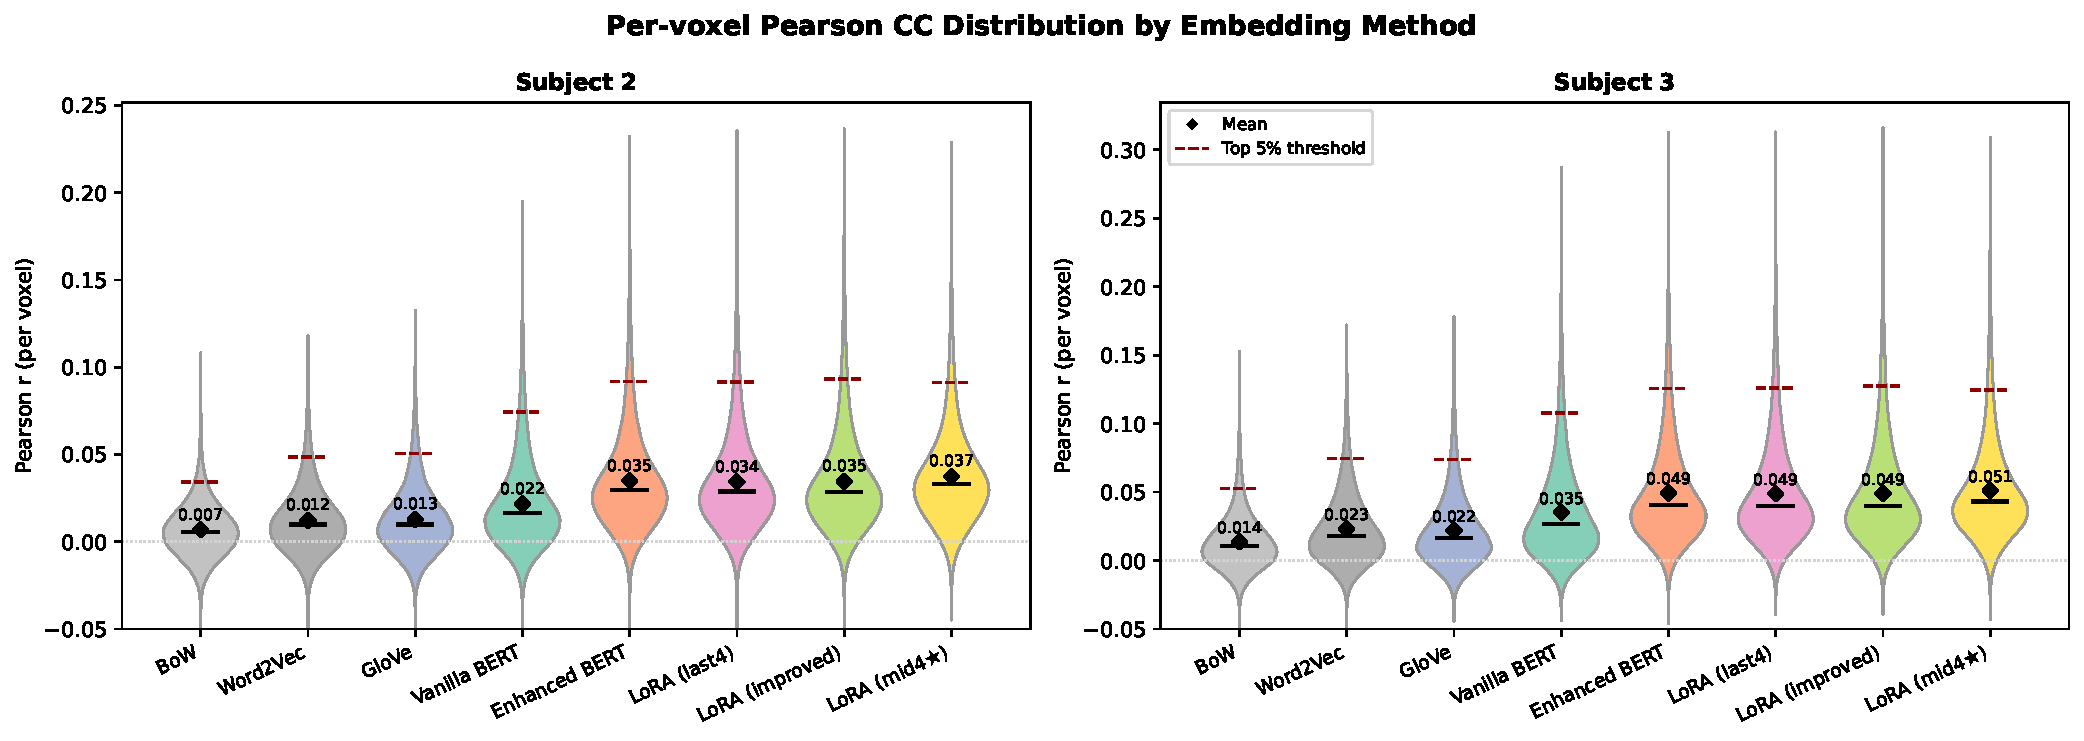
\includegraphics[width=\linewidth]{results/regression/fig1_cc_distributions.pdf}
  \caption{Per-voxel Pearson $r$ distribution for each embedding method,
           shown as violin plots.  Black diamonds ($\blacklozenge$) mark the
           mean; dashed red lines mark the 95th-percentile threshold.
           Left: Subject~2 (94{,}251 voxels).  Right: Subject~3 (95{,}556
           voxels).  Methods are ordered from left to right in increasing
           mean performance.}
  \label{fig:cc_dist}
\end{figure}


\subsection{Statistical Significance of Method Gains}


Figure~\ref{fig:method_prog} summarises the progression quantitatively,
showing the percent gain in mean $r$ over the GloVe baseline for each method
and both subjects.

Every consecutive step in the eight-method hierarchy produces a statistically
significant improvement ($p < 10^{-15}$, paired Wilcoxon signed-rank test on
all ${\sim}94{,}000$ per-voxel differences), with one exception: the transition
from Enhanced BERT to LoRA (last4) is not significant in s2 ($p \approx 1.0$),
consistent with the $<2\%$ numerical gap between those methods.  The
non-contextual tier transitions---BoW$\to$Word2Vec and Word2Vec$\to$GloVe---are
also highly significant, reflecting genuine semantic gains at each step even
among static embeddings.  The gain from LoRA (last4) to LoRA (mid4) is strongly
significant ($p < 10^{-15}$), confirming that the layer-selection
choice---middle layers 5--8 vs.\ final layers 9--12---has a genuine and
reproducible effect on cortical prediction.

Relative to GloVe, LoRA (mid4) achieves $+193\%$ mean-$r$ improvement on s2
and $+133\%$ on s3, while BoW falls $-46\%$/$-37\%$ below GloVe.
The diminishing returns from LoRA (improved) to LoRA (mid4) ($+$8.4\% on s2)
suggest that the architectural change in layer selection dominates over any
refinement in the fine-tuning recipe.

\begin{figure}[H]
  \centering
  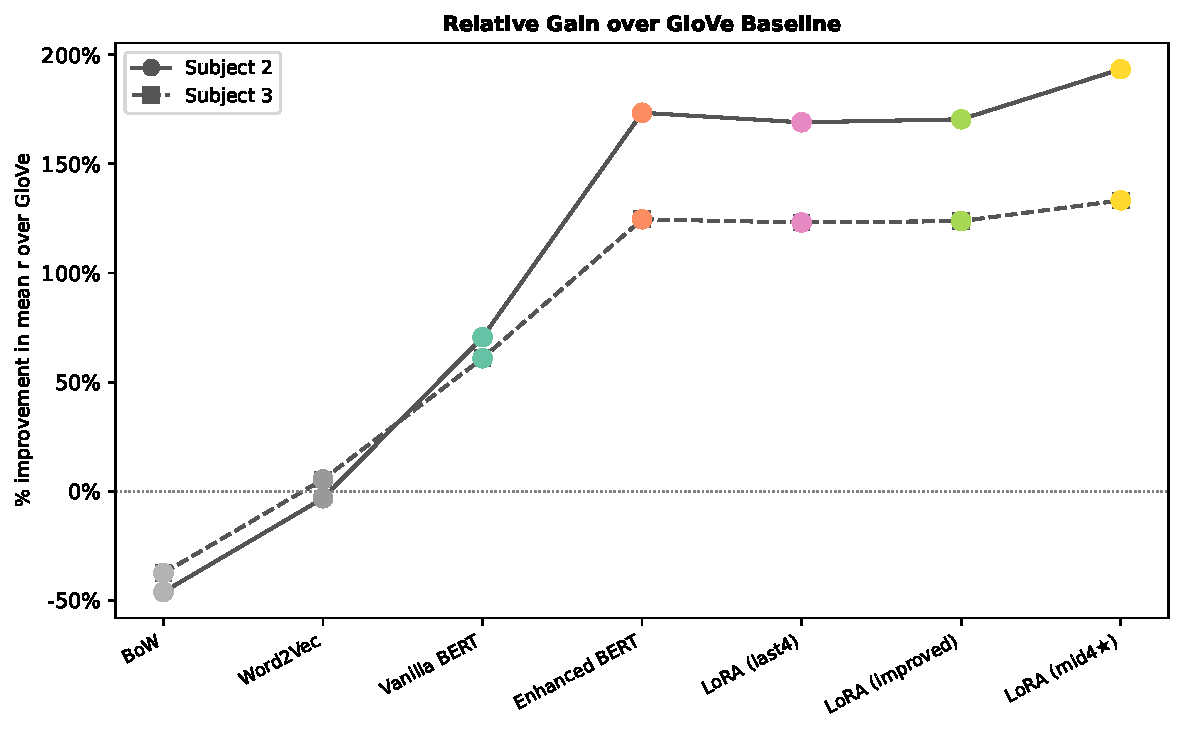
\includegraphics[width=0.8\linewidth]{results/regression/fig2_method_progression.pdf}
  \caption{Percent improvement in mean Pearson $r$ relative to the GloVe
           baseline for each non-GloVe method.  Circles and solid line:
           Subject~2; squares and dashed line: Subject~3.  Coloured dots
           follow the per-method colour scheme used throughout.  Negative
           values (BoW, Word2Vec on s2) indicate that those methods fall
           \emph{below} GloVe; BERT-based methods show large positive gains
           peaking at $+193\%$/$+133\%$ for LoRA (mid4).}
  \label{fig:method_prog}
\end{figure}


\subsection{Inter-Method Voxel-Ranking Correlation}

A natural question is whether different embedding families identify the
\emph{same} language-responsive voxels.  We measure this with the Spearman
rank correlation $\rho$ between per-voxel CC vectors for each pair of methods
within a subject (Figure~\ref{fig:intermethod}).

Four tiers of agreement emerge.
\textbf{(1) Within the non-contextual tier:}
BoW vs.\ Word2Vec ($\rho = 0.51$/$0.64$ on s2/s3) and BoW vs.\ GloVe
($\rho = 0.55$/$0.66$) show only moderate agreement, reflecting that one-hot
counts share some voxel-ranking signal with semantic vectors but miss the bulk
of it.  Word2Vec vs.\ GloVe is substantially higher ($\rho = 0.75$/$0.82$),
consistent with both methods producing semantically comparable 300-d dense
vectors trained on similar large-scale corpora.
\textbf{(2) Non-contextual vs.\ BERT:}
GloVe vs.\ any BERT variant spans $\rho = 0.56$--$0.63$ (s2) and
$0.69$--$0.75$ (s3), indicating that static distributional statistics share a
moderate portion of the brain-predictive signal with contextual representations
but capture a meaningfully different set of language-responsive voxels.
\textbf{(3) Vanilla BERT vs.\ fine-tuned BERT:}
$\rho \approx 0.80$--$0.81$ (s2) and $0.88$ (s3), reflecting the shared
pretrained backbone.  Notably, Enhanced BERT and LoRA (last4) are nearly
indistinguishable in which voxels they predict ($\rho = 0.957$/$0.973$),
confirming that podcast fine-tuning does not meaningfully shift the spatial
prediction pattern when reading from the upper layers.
\textbf{(4) Within the LoRA family:}
LoRA (last4) vs.\ LoRA (improved) yields $\rho = 0.977$/$0.984$, near-perfect
agreement confirming that the refined masking-and-window training recipe makes
negligible difference to which voxels benefit.  LoRA (last4) vs.\ LoRA (mid4),
however, drops to $\rho = 0.866$/$0.909$, a meaningful reduction showing that
changing the extraction layer from 9--12 to 5--8 genuinely redistributes
predictive power to a different set of brain regions---consistent with the
hypothesis that middle BERT layers are more broadly aligned with cortical
language processing than the task-specialised upper layers.

\begin{figure}[htbp]
  \centering
  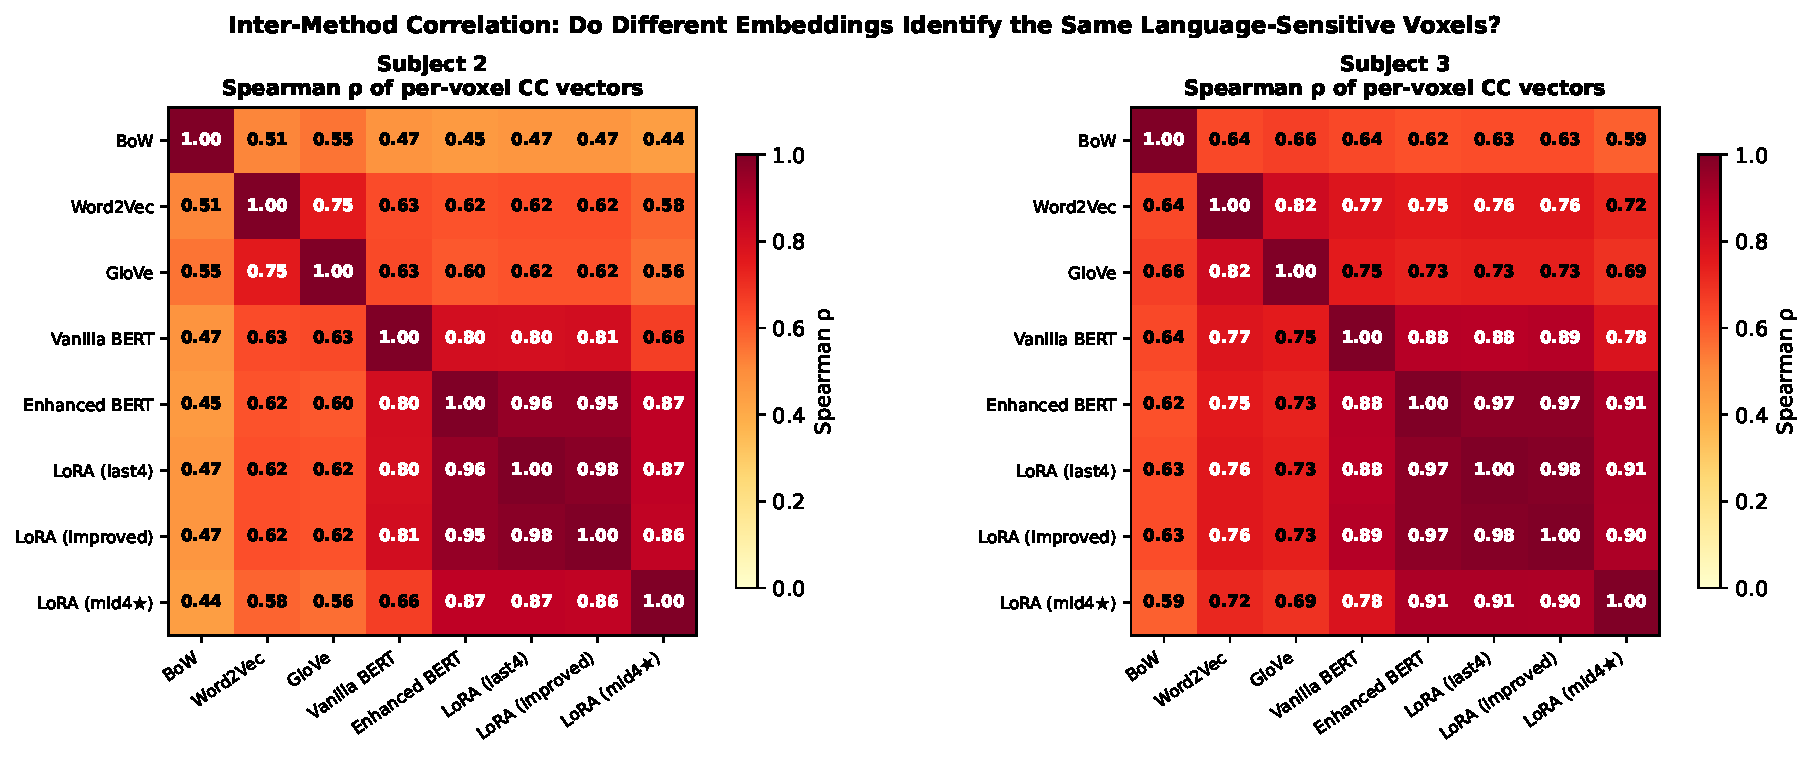
\includegraphics[width=\linewidth]{results/regression/fig3_intermethod_corr.pdf}
  \caption{Spearman rank correlation $\rho$ between per-voxel CC vectors for
           every method pair, computed within each subject.  Higher values mean
           the two methods rank voxels similarly in terms of language
           responsiveness.  Left: Subject~2.  Right: Subject~3.}
  \label{fig:intermethod}
\end{figure}
